\documentclass{article}
\usepackage{graphicx}
\usepackage[utf8]{inputenc}
\usepackage{amsmath, amssymb, latexsym}
\usepackage{neuralnetwork}
\usepackage{multicol}
\usepackage{expl3}

\usepackage{pgfplots}
\usepackage{algorithm}
\usepackage[noend]{algpseudocode}
\usepackage{tikz}
\usepackage{nicefrac}
\pgfplotsset{every axis legend/.append style={
at={(0,0)},
anchor=north east}}
\usetikzlibrary{shapes,positioning,intersections,quotes}
\usetikzlibrary{arrows.meta,
                bending,
                intersections,
                quotes,
                shapes.geometric}
                
\definecolor{darkgreen}{rgb}{0.0, 0.6, 0.0}
\definecolor{darkred}{rgb}{0.7, 0.0, 0.0}
\makeatletter
\def\BState{\State\hskip-\ALG@thistlm}
\makeatother
\title{Week 12}
\begin{document}
\pagenumbering{gobble}
\maketitle
\newpage
\pagenumbering{arabic}

\section*{An alternative view of logistic regression}

As previously stated, the logistic regression hypothesis is as follows:

$$h_{\theta}(x) = \frac{1}{1+e^{-\theta^Tx}}$$

~\\
We have an example in which $y = 1$. We expect that $h_{\theta}(x)$ is close to 1.

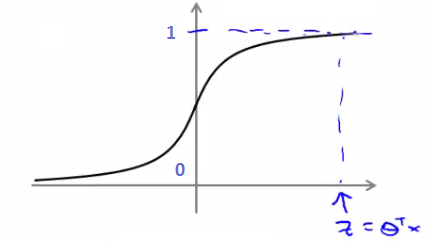
\includegraphics[width=0.5\textwidth]{resources/sigmoid2}

~\\
When you look at the cost function, you'll see that each example contributes a term like the one below to the total cost function.

$$-(ylogh_{\theta}(x)+(1-y)log(1-h_{\theta}(x)))$$

~\\
After plugging in the hypothesis function $h_{\theta}(x)$, you obtain an enlarged cost function equation:

$$-ylog\frac{1}{1+e^{-\theta^Tx}}-(1-y)log(1-\frac{1}{1+e^{-\theta^Tx}})$$

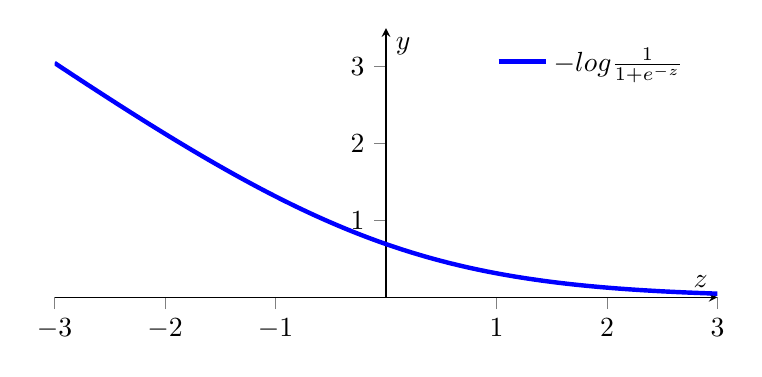
\begin{tikzpicture}
  \begin{axis}[
      axis x line=middle,
      axis y line=middle,
      width=10cm,
      height=5cm,
      xmin=-3,   % start the diagram at this x-coordinate
      xmax= 3,   % end   the diagram at this x-coordinate
      ymin=0,   % start the diagram at this y-coordinate
      ymax= 3.5,   % end   the diagram at this y-coordinate
      xlabel=$z$,
      ylabel=$y$,
      legend cell align=left,
      legend pos=north east,
      legend style={draw=none},
      tick align=outside,
      enlargelimits=false]
    % plot the function

    \addplot[domain=-3:3, blue, ultra thick,samples=500] {-ln(1/(1+exp(-x)))};
    \legend{$-log \frac{1}{1+e^{-z}}$}
  \end{axis}
\end{tikzpicture}

\begin{itemize}
  \item As a result, if z is large, the cost is small.
  \item If z is 0 or negative, however, the cost contribution is large..
  \item This is why, when logistic regression encounters a positive case, it attempts to make $\theta^Tx$ a very big term.
\end{itemize}

\section*{SVM cost functions from logistic regression cost functions}

\begin{itemize}
  \item Instead of a curved line, draw two straight lines (magenta) to approximate the logistic regression y = 1 function.
  \item Flat when cost is 0.
  \item Straight growing line after 1.
  \item So this is the new y=1 cost function, which provides the SVM with a computational advantage and makes optimization easier.
\end{itemize}

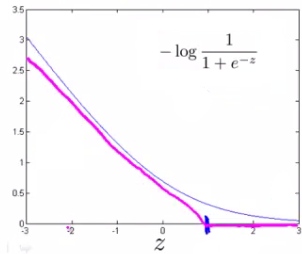
\includegraphics[width=0.5\textwidth]{resources/svm_cost}

~\\
Logistic regression cost function:

$$J(\theta) = -\frac{1}{m} \sum_{i=1}^{m}[ y^{(i)} log h_{\theta}(x^{(i)}) + (1- y^{(i)})log(1 - h_{\theta}(x^{(i)}))] +  \frac{\lambda}{2m} \sum_{j=1}^{m} \theta_j^2$$

~\\
For the SVM we take our two logistic regression $y=1$ and $y=0$ terms described previously and replace with $cost_1(\theta^Tx)$ and $cost_0(\theta^Tx)$.

$$J(\theta) = -\frac{1}{m} \sum_{i=1}^{m}[ y^{(i)} cost_1(\theta^Tx^{(i)}) + (1- y^{(i)}) cost_0(\theta^Tx^{(i)})] +  \frac{\lambda}{2m} \sum_{j=1}^{m} \theta_j^2$$

~\\
Which can be rewritten as:

$$J(\theta) = C \sum_{i=1}^{m}[ y^{(i)} cost_1(\theta^Tx^{(i)}) + (1- y^{(i)}) cost_0(\theta^Tx^{(i)})] +  \frac{1}{2} \sum_{j=1}^{m} \theta_j^2$$

\begin{itemize}
  \item Large C gives a hypothesis of low bias high variance $->$ overfitting
  \item Small C gives a hypothesis of high bias low variance $->$ underfitting
\end{itemize}

\section*{Large margin intuition}
\begin{itemize}
  \item So, given that we're aiming to minimize CA + B.
  \item Consider the following scenario: we set C to be really large.
  \item If C is large, we will choose an A value such that A equals zero.
  \item If y = 1, then we must find a value of $\theta$ so that $\theta^Tx$ is larger than or equal to 1 in order to make our "A" term 0.
  \item If y = 0, then we must find a value of $\theta$ so that $\theta^Tx$ is equal to or less than -1 in order to make our "A" term 0.
  \item So we're minimizing B, under the constraints shown below:
\end{itemize}

$$min\ \frac{1}{2} \sum_{j=1}^{m} \theta_j^2$$

$$\theta^Tx^{(i)} \geq 1 \quad if\ y^{(i)}=1$$
$$\theta^Tx^{(i)} \leq 1 \quad if\ y^{(i)}=0$$

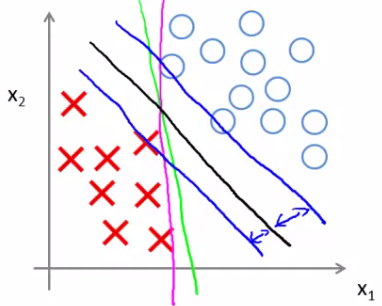
\includegraphics[width=0.5\textwidth]{resources/large_dist}

\begin{itemize}
  \item The green and magenta lines represent functional decision limits that might be selected using logistic regression. However, they are unlikely to generalize effectively.
  \item The black line, on the other hand, is the one picked by the SVM as a result of the optimization graph's safety net. Stronger separator.
  \item That black line has a greater minimum distance (margin) than any of the training samples.
\end{itemize}

\section*{SVM decision boundary}

Assume we only have two features and $\theta_0=0$. Then we can rewrite th expression for minimizing B as follows:

$$\frac{1}{2}(\theta_1^2 + \theta_2^2) =\frac{1}{2}(\sqrt{\theta_1^2 + \theta_2^2})^2 = \frac{1}{2}||\theta||^2$$

\begin{itemize}
  \item Given this, what are $\theta^Tx$ parameters doing?
  \item Assume we have just one positive training example (red cross below).
  \item Assume we have our parameter vector and plot it on the same axis.
  \item The following question asks what the inner product of these two vectors is.
\end{itemize}

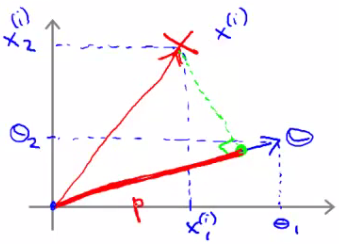
\includegraphics[width=0.5\textwidth]{resources/svm_vectors}

~\\
$p$, is in fact $p^i$, because it's the length of $p$ for example $i$.

$$\theta^Tx^{(i)} = p^i \cdot ||\theta||$$

$$min\ \frac{1}{2} \sum_{j=1}^{m} \theta_j^2 = \frac{1}{2} ||\theta||^2$$

$$p^{(i)} \cdot ||\theta|| \geq 1 \quad if\ y^{(i)}=1$$
$$p^{(i)} \cdot ||\theta|| \leq 1 \quad if\ y^{(i)}=0$$

\section*{Adapting SVM to non-linear classifiers}

\begin{itemize}
  \item We have a training set.
  \item We want to find a non-linear boundary.
\end{itemize}

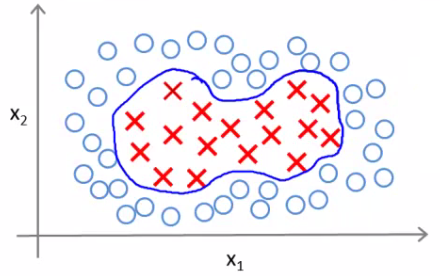
\includegraphics[width=0.5\textwidth]{resources/non_linear_boundary}

\begin{itemize}
  \item Define three features in this example (ignore $x_0$).
  \item Have a graph of $x_1$ vs. $x_2$ (don't plot the values, just define the space).
  \item Pick three points.
\end{itemize}

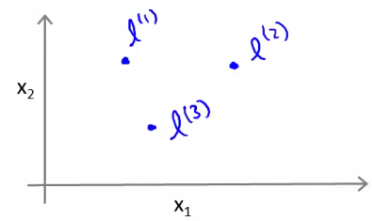
\includegraphics[width=0.5\textwidth]{resources/landmarks}

\begin{itemize}
  \item These points $l^1$, $l^2$, and $l^3$, were chosen manually and are called landmarks.
  \item Kernel is the name given to the similarity function between $(x, l^i)$.
\end{itemize}

$$f_1 = k(X, l^1) = exp(- \frac{||x-l^{(1)}||^2}{2\sigma^2})$$

\begin{itemize}
  \item Large $\sigma^2$ - $f$ features vary more smoothly - higher bias, lower variance.
  \item Small $\sigma^2$ - $f$ features vary abruptly - low bias, high variance.
  \item With training examples x we predict "1" when: $\theta_0+\theta_1f_1+\theta_2f_2+\theta_3f_3 \geq 0$
  \item Let's say that: $\theta_0 = -0.5,\ \theta_1=1,\ \theta_2=1,\ \theta_3=0$
  \item Given our placement of three examples, what happens if we evaluate an example at the magenta dot below?
\end{itemize}

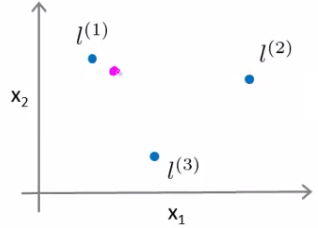
\includegraphics[width=0.5\textwidth]{resources/landmarks_magneta}

\begin{itemize}
  \item We can see from our formula that f1 will be close to 1, whereas f2 and f3 will be close to 0.
  \item We have: $-0.5+1\cdot1+0\cdot1+0\cdot0 \geq 0$.
  \item The inequality holds. We predict 1.
  \item If we had another point far away from all three. The inequality wouldn't hold. As a result, we would predict 0.
\end{itemize}

\section*{Choosing the landmarks}

\begin{itemize}
  \item Take the training data. Vectors X and Y, both with m elements.
  \item As a result, you'll wind up having m landmarks. Each training example has one landmark per location.
  \item So we just cycle over each landmark, determining how close $x^i$ is to that landmark. Here we are using the kernel function.
  \item Take these m features $(f_1, f_2 ... f_m)$ group them into an $[m +1 \times 1]$ dimensional vector called $f$.
\end{itemize}

\section*{Kernels}

\begin{itemize}
  \item Linear kernel: no kernel, no $f$ vector. Predict $y=1$ if $(\theta^Tx) \geq 0$.
  \item Not all similarity functions you develop are valid kernels. Must satisfy Merecer's Theorem.
  \item Polynomial kernel.
  \item String kernel.
  \item Chi-squared kernel.
  \item Histogram intersection kernel.
\end{itemize}

\section*{Logistic regression vs. SVM}

\begin{itemize}
  \item Use logistic regression or SVM with a linear kernel if n (features) is much greater than m (training set).
  \item If n is small and m is intermediate, the Gaussian kernel is suitable.
  \item With a Gaussian kernel, SVM will be sluggish if n is small and m is large. Use logistic regression or SVM with a linear kernel.
  \item A lot of SVM's power is using diferent kernels to learn complex non-linear functions.
  \item Because SVM is a convex optimization problem, it gives a global minimum.
\end{itemize}

\end{document}
